\documentclass[compress]{beamer}
\usefonttheme[onlymath]{serif}
\usepackage{ctex}
\usepackage{bm}
\usepackage{subfig}
\usepackage{diagbox}
\usepackage{algorithm}
\usepackage{algorithmic}
\usepackage{color}

%\usecolortheme{rose}
%\usecolortheme{seahorse}
\setbeamertemplate{navigation symbols}{} % remove navigation symboles
\setbeamertemplate{headline}{} % remove headline

% move the style of headline to footline
\setbeamertemplate{footline}
{%
  \begin{beamercolorbox}[colsep=1.5pt]{upper separation line head}
  \end{beamercolorbox}
  \begin{beamercolorbox}{section in head/foot}
    \vskip2pt\insertnavigation{\paperwidth}\vskip2pt
  \end{beamercolorbox}%
  \begin{beamercolorbox}[colsep=1.5pt]{lower separation line head}
  \end{beamercolorbox}
}

% assign a dot for each frame instead of each subsection
\usepackage{remreset}
\makeatletter
\@removefromreset{subsection}{section}
\makeatother
\setcounter{subsection}{1}

% unfold step by step
\beamerdefaultoverlayspecification{<+->}

\DeclareMathOperator*{\argmin}{argmin}
\DeclareMathOperator*{\argmax}{argmax}
\floatname{algorithm}{算法}
\renewcommand{\algorithmicrequire}{\textbf{输入:}}
\renewcommand{\algorithmicensure}{\textbf{输出:}}


\title{基于SSD的HDD缓存系统研究}
\author{闫林}
\institute{
计算机学院\\
西安电子科技大学\\
\vspace{5mm}
指导教师:刘凯教授
}

\begin{document}

\begin{frame}[plain] % use plain since we donot want footline on the title page
  \titlepage
\end{frame}

\AtBeginSection{
  \begin{frame}
    \frametitle{目录}
    \tableofcontents[currentsection]
  \end{frame}
}

%---------------------------------------------------------------
\section{研究背景}
%---------------------------------------------------------------
\begin{frame}{背景介绍}
固态硬盘有着体积小、功耗低以及访问速度快等优势。但固态硬盘的高昂价格和相对较低的存储密度,使其难以在短时间内完全取代传统的机械硬盘。
\begin{itemize}
    \item 固态硬盘的价格从2006的3美元/GB,跌至2014年的0.67美元/GB,但和机械硬盘0.09美元/GB仍存较大差距。通过固态硬盘价格的历史下降速度可以推算出到2020年其价格约为0.14美元/GB,同样计算方法得出的机械硬盘价格将会是0.03美元/GB。
\end{itemize}
\end{frame}

\begin{frame}{固态硬盘的应用}
在许多存储中心,同时部署固态硬盘和机械硬盘。只有部分固态硬盘的存储空间被用作存储。
\end{frame}

%---------------------------------------------------------------
\section{问题提出和解决方案}
%---------------------------------------------------------------
\begin{frame}{问题提出}
\begin{itemize}
    \item 如何发挥固态硬盘的高性能?
    \item 或者是,如何充分利用空闲的固态盘存储空间?
\end{itemize}
\end{frame}

\begin{frame}{解决方案}
论文课题提出了一种基于固态硬盘的机械硬盘缓存系统,使用固态硬盘的存储空间作为机械硬盘的缓存,通过实现多种缓存管理算法,提升存储系统的IO性能。
\end{frame}

\section{研究现状}

\begin{frame}{研究成果}
\begin{itemize}
    \item Mac的Fusion Drive使用LVM实现了基于SSD的HDD缓存。
    \item Linux操作系统下存在dmcache(redhat), bcache(kernel)和flashcache(Facebook)几种基于SSD的缓存技术的开源实现。
    \item Windows系统自带的ReadyBoost是一种解决方案,但其只支持闪存(NAND 存储)设备作为缓存,如果驱动器采用的固态硬盘(SSD),ReadyBoost将不可用。
    \item 论文实现的缓存系统将会弥补ReadyBoost的不足。
\end{itemize}
\begin{figure}
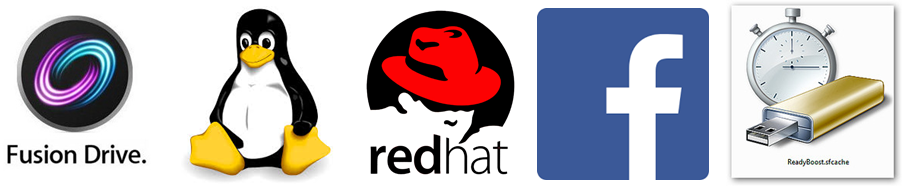
\includegraphics[width=0.5\linewidth]{./fig/research-status}
\end{figure}
\end{frame}

%---------------------------------------------------------------
\section{本文方法}
%---------------------------------------------------------------
\begin{frame}{缓存系统架构}
\begin{figure}
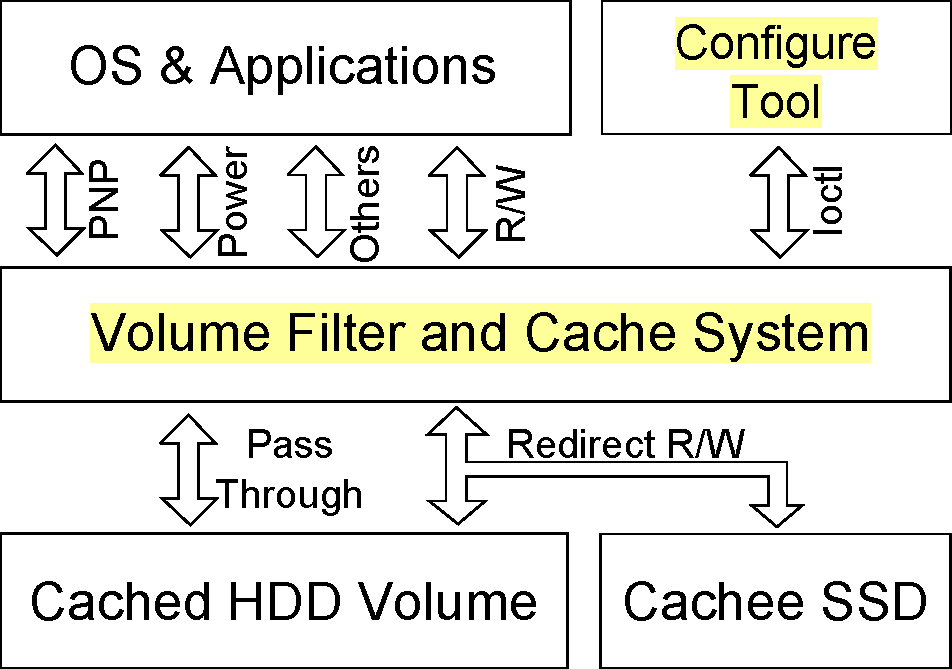
\includegraphics[width=0.8\linewidth]{./fig/sys-overview}
\end{figure}
\end{frame}

\begin{frame}{工作内容}
\begin{itemize}
\item 存储卷过滤器驱动
    \begin{itemize}
    \item Windows WDM 驱动模型开发
    \end{itemize}
\item 缓存系统
    \begin{itemize}
    \item 页面替换算法设计
    \item 回写策略设计
    \item 映射策略设计
    \end{itemize}
\item 配置工具
    \begin{itemize}
    \item 通过IOCTL命令与驱动程序进行交互
    \end{itemize}
\end{itemize}
\end{frame}

\begin{frame}{驱动模块组成}
\begin{figure}
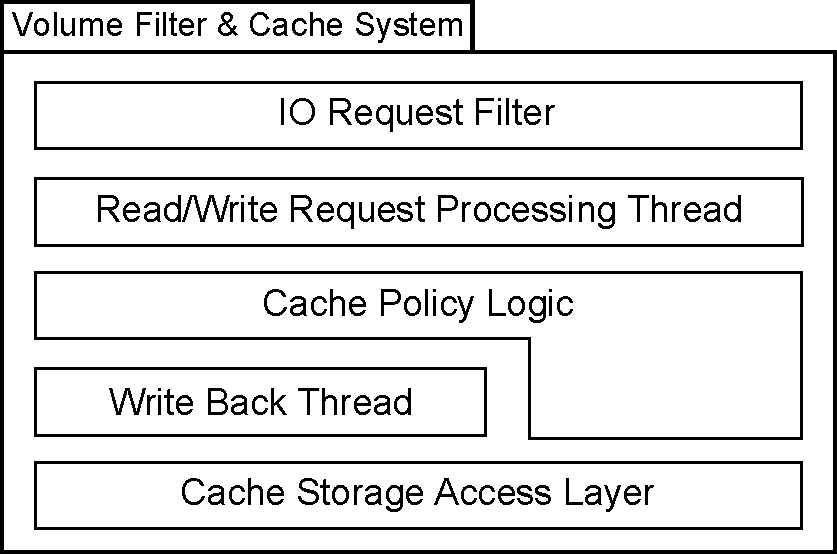
\includegraphics[width=0.8\linewidth]{../graph/sys-flt-arch}
\end{figure}
\end{frame}

\begin{frame}{IO Request Filter}
    \begin{columns}
    \begin{column}{0.5\textwidth}
        \begin{figure}
        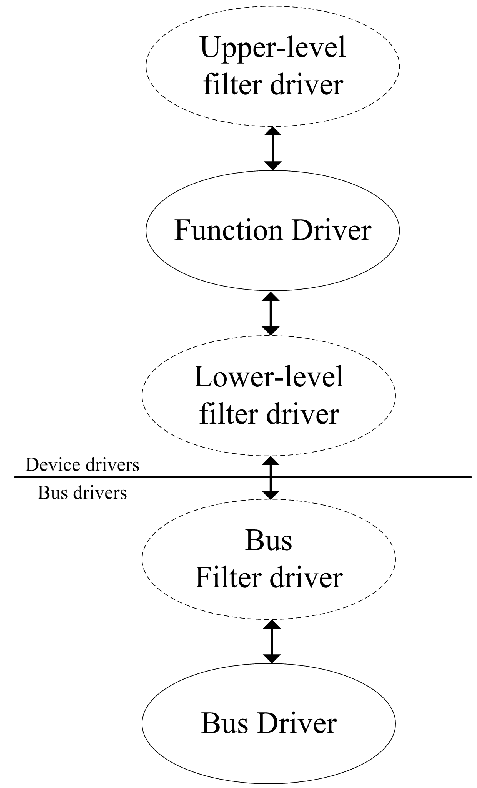
\includegraphics[width=0.8\textwidth]{../graph/io-stack-filter}
        \end{figure}
    \end{column}
    \begin{column}{0.5\textwidth}
        使用Windows系统WDM驱动程序模型完成的过滤器类型驱动。

        Windows驱动程序分三类:
        \begin{itemize}
        \item 功能驱动。
        \item 总线驱动。
        \item 过滤器驱动:过滤上两类驱动间的消息传递IRP。
        \end{itemize}

        过滤器驱动也分三类。
        系统实现了上层过滤器驱动。
    \end{column}
    \end{columns}
\end{frame}

\begin{frame}{Read/Write Processing Thread}
    \begin{columns}
    \begin{column}{0.5\textwidth}
        \begin{figure}
        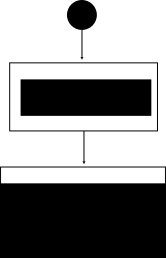
\includegraphics[width=0.4\textwidth]{../graph/df-rw}
        \end{figure}
    \end{column}
    \begin{column}{0.5\textwidth}
        \begin{figure}
        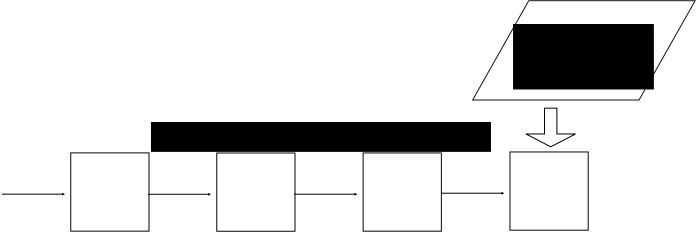
\includegraphics[width=1.0\textwidth]{../graph/df-rw-thread}
        \end{figure}
    \end{column}
    \end{columns}
过滤器驱动程序会将读写请求加入等待队列中,并返回一个pending状态,表示正在处理请求。读写线程检测到队列不为空时,便通过和缓存系统交互,处理每个读写请求。
\end{frame}

\begin{frame}{缓存系统逻辑}
缓存系统
\begin{itemize}
\item 缓存页面替换算法
\item 缓存索引数据结构
\item 缓存块映射策略
\item 回写策略
\end{itemize}
\end{frame}

\begin{frame}{缓存系统:替换算法}
\begin{itemize}
\item 替换算法的功能是:缓存已经满时,决定哪些缓存块会被替换掉。
\item LRU(Least Recently Used)
\item LFU(Least Frequently Used)
\item 论文使用一种综合考虑访问时间和使用频度的替换算法,该算法实现简单,且结果表明命中率优于LRU和LFU替换算法。
\end{itemize}
\end{frame}

\begin{frame}{缓存系统:替换算法}
\begin{figure}
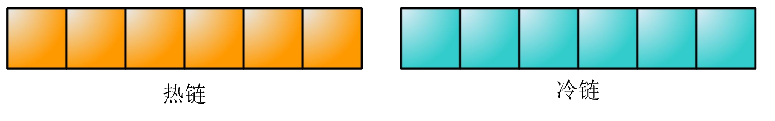
\includegraphics[width=0.6\linewidth]{../graph/replace-algo-1}
\end{figure}
\begin{figure}
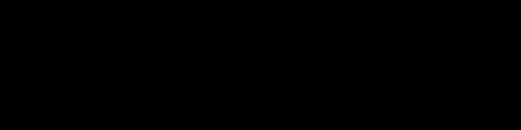
\includegraphics[width=0.6\linewidth]{../graph/replace-algo-2}
\end{figure}
缓存块首先会被加入到冷链表的热端,在运行过程中会统计每个缓存块的访问计数(初始为 1)。如果某个缓存块被访问,该缓存块无论在冷链还是热链都会被移动到该链表的热端,并且访问计数增加 1。
\end{frame}

\begin{frame}{缓存系统:替换算法}
\begin{figure}
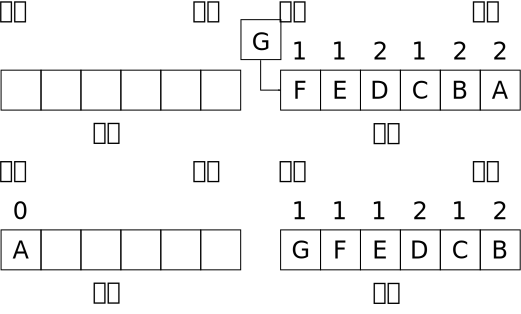
\includegraphics[width=0.6\linewidth]{../graph/replace-algo-3}
\end{figure}
当冷链表已满,而又要加入新的缓存块时。新的缓存块仍旧会被加入到冷链的热端。算法判断被移出缓存块的引用计数,如果其引用计数大于等于2,则清零其引用计数,并加入到热链表的热端;否则缓存块空间将会被释放。
\end{frame}

\begin{frame}{缓存系统:替换算法}
\begin{figure}
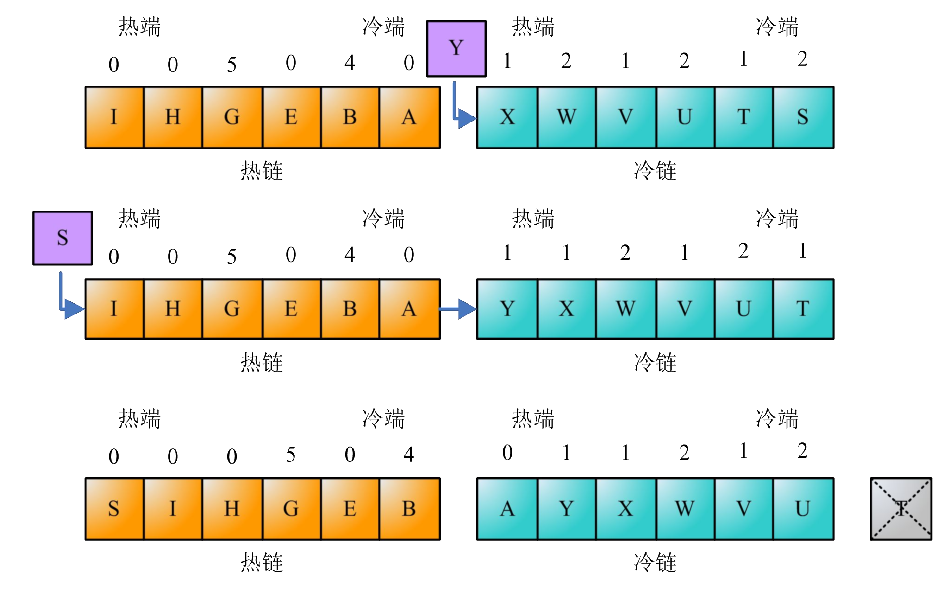
\includegraphics[width=0.6\linewidth]{../graph/replace-algo-4}
\end{figure}
当热链表中也不存在空闲空间时,加入新缓存块,热链表冷端的缓存一样会被换出。从热链中被换出的缓存块的引用计数会被清零,然后加入到冷链表的热端,如此循环直到达到稳定。
\end{frame}

\begin{frame}{缓存系统:替换算法}
\begin{itemize}
\item 本替换算法的核心思想是:冷、热链表内部完成LRU替换算法;冷、热链表之间完成LFU替换算法。
\item 单独观察冷或热链表,实质就是一个LRU算法管理的链表。缓存块在两个链表之间移动时,考虑到了访问频度的因素,这一点则反映了LFU替换算法的思想。
\end{itemize}
\end{frame}

\begin{frame}{缓存系统:映射策略}
映射策略指的是从主存到缓存的映射方式,直接决定了缓存的查询方式。
论文使用了全相联映射的方式,缓存中的每一块都可映射给将主存中的任意一块数据。
\begin{figure}
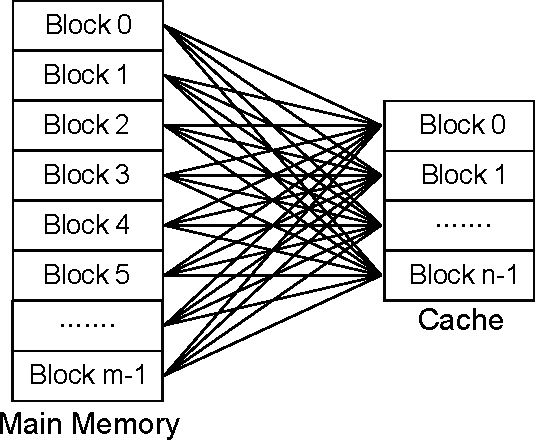
\includegraphics[width=0.6\linewidth]{../graph/cache-map-2}
\end{figure}
\end{frame}

\begin{frame}{缓存系统:映射策略}
全相联映射的优点是空间利用灵活,缺点是必须要使用辅助的查找数据结构建立索引。

论文使用B+树索引数据结构。

B+树所有叶子节点在同一层上,只有叶子节点储存数据。
\begin{figure}
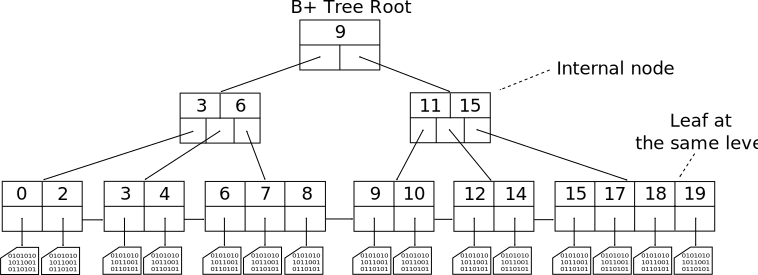
\includegraphics[width=0.9\linewidth]{../graph/bplus-tree}
\end{figure}
\end{frame}

\begin{frame}{缓存系统:回写策略}
\begin{itemize}
\item 对于应用程序的写请求,回写策略决定了直接将写请求应用到主存储器上还是延迟后再进行回写更新。
\item 本论文的SSD缓存系统提供了写穿法(Write Through)、写回法(Write Back)两种回写策略的实现。
\end{itemize}
\begin{figure}
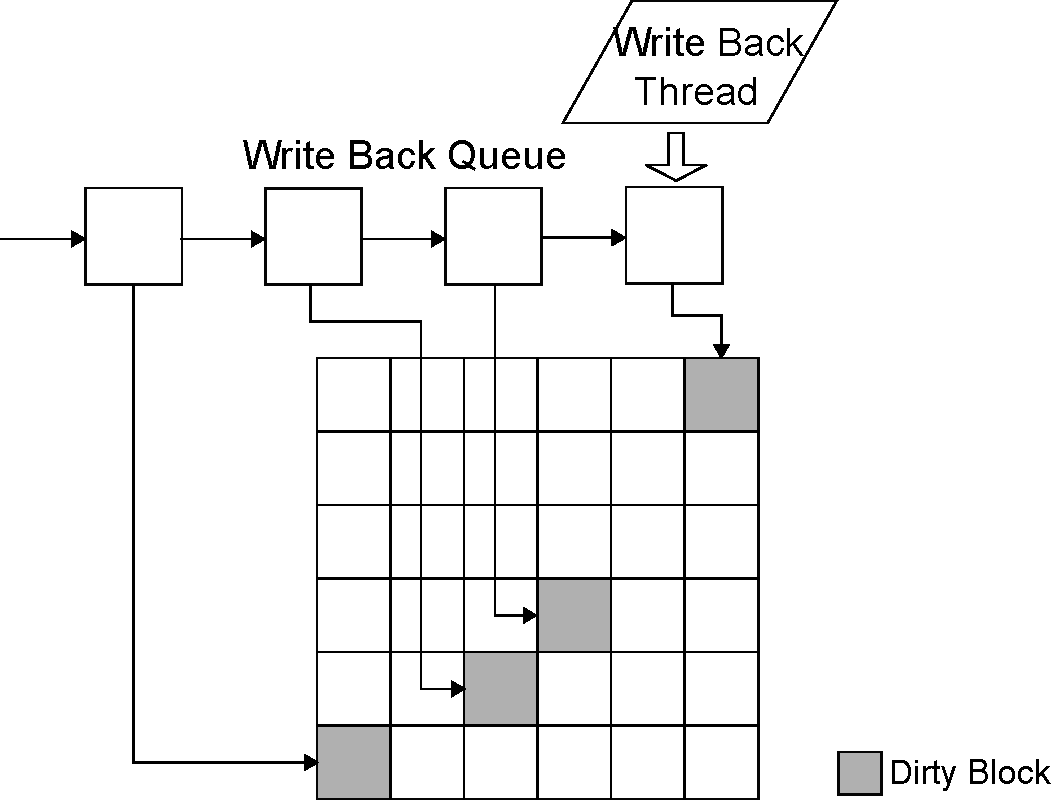
\includegraphics[width=0.6\linewidth]{../graph/write-back-queue}
\end{figure}
\end{frame}

\begin{frame}{缓存系统:回写策略(写穿)}
    \begin{columns}
    \begin{column}{0.5\textwidth}
        \begin{figure}
        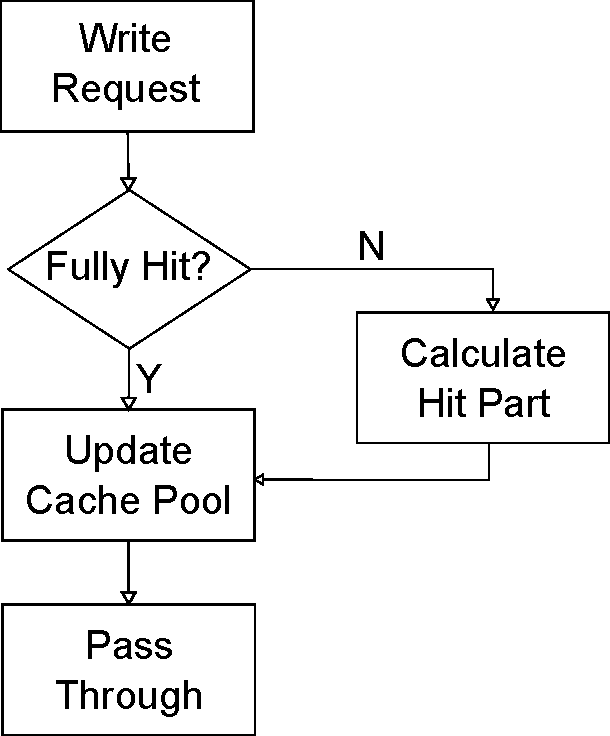
\includegraphics[width=0.6\textwidth]{../graph/write-through}
        \end{figure}
    \end{column}
    \begin{column}{0.5\textwidth}
        \begin{itemize}
        \item 写穿法对于接收到的写请求,同时应用于机械硬盘和固态硬盘缓存。
        \item 优点:无需考虑断电造成的数据丢失问题。
        \item 缺点:无法提升应用程序的写操作的IO性能,相反的,还会造成写性能一定程度的降低。
        \end{itemize}
    \end{column}
    \end{columns}
\end{frame}

\begin{frame}{缓存系统:回写策略(写回)}
\begin{itemize}
\item 写回法对于接收到的写请求,只将写操作应用于固态硬盘缓存,更新后立即完成写操作请求。回写线程在延迟一定时间后同步机械硬盘数据。
\item 优点:可以提升写操作的性能。
\item 缺点:有断电造成的数据丢失风险。
\end{itemize}

\begin{block}{触发条件}
数据最终还是要被写回。
\begin{itemize}
\item 定时刷新。
\item 定量刷新。
\item 经测试,定量刷新性能优于定时刷新。
\end{itemize}
\end{block}
\end{frame}

\begin{frame}{缓存系统:回写策略(写回)}
    \begin{columns}
    \begin{column}{0.5\textwidth}
        \begin{figure}
        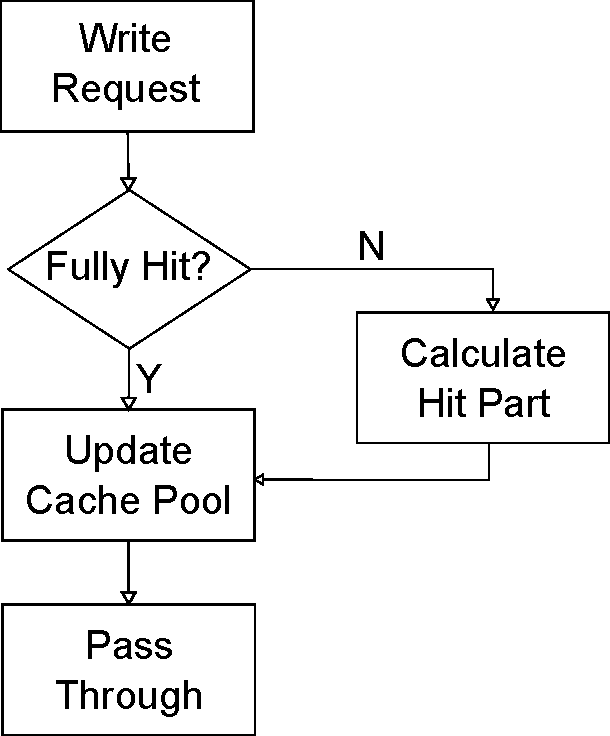
\includegraphics[width=0.6\textwidth]{../graph/write-through}
        \end{figure}
    \end{column}
    \begin{column}{0.5\textwidth}
        论文使用了定量刷新的方式管理回写。
        三个触发条件:
        \begin{itemize}
        \item 队列已满
        \item ‘写回所有’
        \item ‘终止线程’
        \end{itemize}
    \end{column}
    \end{columns}
\end{frame}

\begin{frame}{配置工具}
\begin{itemize}

\item start   disk\_number   volume\_number

开启对某个存储卷的缓存

\item stop   disk\_number   volume\_number

停止对某个存储卷的缓存

\item stat   disk\_number   volume\_number

打印信息统计信息。读写次数,读写命中次数,缓存使用

\item verbose

输出所有调试信息

\item quiet

关闭所有调试信息输出

\end{itemize}
\end{frame}

%---------------------------------------------------------------
\section{系统测试}
%---------------------------------------------------------------
\begin{frame}{测试平台和工具}

\begin{itemize}
\item 测试平台

操作系统 Microsoft Windows Server 2008 R2

机械硬盘 250GB seagate st9250320as

固态硬盘 120GB crucial ct120m500ssd1

驱动程序开发工具 Microsoft Windows Driver Kit 7600.1

应用程序开发工具 Microsoft Visual Studio 2008

性能测试工具 FIO Disk Benchmarking 2.0.8

\item 测试分为正确性验证和性能测试两部分
\end{itemize}
\end{frame}

\begin{frame}{正确性验证}
\begin{itemize}
\item 使用chkdsk工具,验证缓存系统不会导致数据损坏或丢失。
\item 验证步骤
\begin{enumerate}
\item 加载缓存系统驱动程序。
\item 配置工具开启对某个存储卷的缓存。
\item 使用性能测试工具FIO测试读写性能。
\item 停止对存储卷的缓存。
\item 卸载缓存驱动程序。
\item 使用chkdsk检测被缓存的存储卷。
\end{enumerate}
\item FIO运行中会产生许多临时文件,chkdsk命令未检测出问题,说明缓存系统通过了正确性验证。
\end{itemize}
\end{frame}

\begin{frame}{性能测试}
\begin{itemize}
\item 测试工具FIO
\end{itemize}
FIO是一款基于GPLv2协议开源的、主要用于测试存储设备的性能和压力上限的性能测试工具。
\begin{block}{测试参数}
size=2000MB                // 机械硬盘2G,SSD缓存200M

numjobs=4                  // 读写线程数目

iodepth=8                  // 并发异步IO请求个数上限

rw=[randrw, randread, randwrite]  // 读写类型

runtime=1000                      // 运行时长

random\_distribution=zipf:1.2     // 读写位置分布
\end{block}
\end{frame}

\begin{frame}{性能测试结果}
\begin{figure}
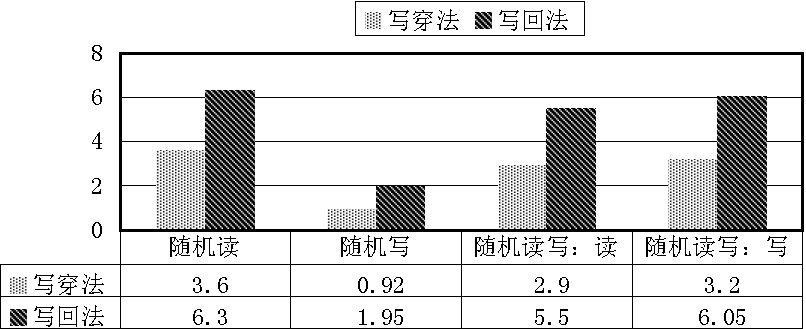
\includegraphics[width=0.7\textwidth]{../graph/enhance-rate}
\end{figure}
缓存系统的存在从一定程度带来了HDD随机读、随机写的性能提升。相较于写穿法,写回法对存储系统的读写性能提升效果更为明显。
\end{frame}

\begin{frame}{与FancyCache比较}
    \begin{table}
    \centering
    \caption{随机读速度比较(KB/s)}
    \begin{tabular}{|c|c|c|}
    \hline
    \diagbox{块大小(KB)}{缓存系统} & 本论文的 & FancyCache \\
    \hline 4  & 2970 & 2508 \\
    \hline 16 & 9821 & 10254 \\
    \hline 64 & 32857 & 51833 \\
    \hline
    \end{tabular}
    \end{table}
\end{frame}
\begin{frame}{与FancyCache比较}
    \begin{table}
    \centering
    \caption{随机写速度比较(KB/s)}
    \begin{tabular}{|c|c|c|}
    \hline
    \diagbox{块大小(KB)}{缓存系统} & 本论文的 & FancyCache \\
    \hline 4  & 2970 & 3021 \\
    \hline 16 & 9821 & 9982 \\
    \hline 64 & 32857 & 32258 \\
    \hline
    \end{tabular}
    \end{table}
\end{frame}

\begin{frame}{展望}
\begin{itemize}
\item 结合固态硬盘特性的性能优化
\item 面向特殊场景的混合存储系统的研究
\item 使用实时压缩算法提高缓存的空间利用率
\end{itemize}
\end{frame}


\section{参考文献}
\begin{frame}[fragile, allowframebreaks]{参考文献}
\begin{thebibliography}{10}
\setbeamertemplate{bibliography item}[text]

\bibitem{bordes2005fast}
Bordes A, Ertekin S, Weston J, \textit{et al.} Fast kernel classifiers with online and active learning[J]. The Journal of Machine Learning Research, 2005, 6: 1579-1619.

\end{thebibliography}
\end{frame}

\end{document}
